\documentclass[12pt]{scrartcl}
\usepackage[sexy]{james}
\usepackage[noend]{algpseudocode}
\setlength{\marginparwidth}{2cm}
\usepackage{graphicx}
\usepackage{answers}
\usepackage{array}
\usepackage{tikz}
\newenvironment{allintypewriter}{\ttfamily}{\par}
\usepackage{listings}
\usepackage{xcolor}
\usetikzlibrary{arrows.meta}
\usepackage{color}
\usepackage{mathtools}
\newcommand{\U}{\mathcal{U}}
\newcommand{\E}{\mathbb{E}}
\usetikzlibrary{arrows}
\Newassociation{hint}{hintitem}{all-hints}
\renewcommand{\solutionextension}{out}
\renewenvironment{hintitem}[1]{\item[\bfseries #1.]}{}
\renewcommand{\O}{\mathcal{O}}
\declaretheorem[style=thmbluebox,name={Chinese Remainder Theorem}]{CRT}
\renewcommand{\theCRT}{\Alph{CRT}}
\setlength\parindent{0pt}
\usepackage{sansmath}
\usepackage{pgfplots}

\usetikzlibrary{automata}
\usetikzlibrary{positioning}  %                 ...positioning nodes
\usetikzlibrary{arrows}       %                 ...customizing arrows
\newcommand{\eqdef}{=\vcentcolon}
\newcommand{\tr}{{\rm tr\ }}
\newcommand{\im}{{\rm Im\ }}
\newcommand{\spann}{{\rm span\ }}
\newcommand{\Col}{{\rm Col\ }}
\newcommand{\Row}{{\rm Row\ }}
\newcommand{\dint}{\displaystyle\int}
\newcommand{\dt}{\ {\rm d }t}
\newcommand{\PP}{\mathbb{P}}
\newcommand{\horizontal}{\par\noindent\rule{\textwidth}{0.4pt}}
\usepackage[top=3cm,left=3cm,right=3cm,bottom=3cm]{geometry}
\newcommand{\mref}[3][red]{\hypersetup{linkcolor=#1}\cref{#2}{#3}\hypersetup{linkcolor=blue}}%<<<changed

\tikzset{node distance=4.5cm, % Minimum distance between two nodes. Change if necessary.
         every state/.style={ % Sets the properties for each state
           semithick,
           fill=cyan!40},
         initial text={},     % No label on start arrow
         double distance=4pt, % Adjust appearance of accept states
         every edge/.style={  % Sets the properties for each transition
         draw,
           ->,>=stealth',     % Makes edges directed with bold arrowheads
           auto,
           semithick}}


% Start of document.
\newcommand{\sep}{\hspace*{.5em}}

\pgfplotsset{compat=1.18}
\begin{document}
\title{MATH410: Homework 3}
\author{James Zhang\thanks{Email: \mailto{jzhang72@terpmail.umd.edu}}}
\date{\today}

\definecolor{dkgreen}{rgb}{0,0.6,0}
\definecolor{gray}{rgb}{0.5,0.5,0.5}
\definecolor{mauve}{rgb}{0.58,0,0.82}

\lstset{frame=tb,
  language=Java,
  aboveskip=3mm,
  belowskip=3mm,
  showstringspaces=false,
  columns=flexible,
  basicstyle={\small\ttfamily},
  numbers=left,
  numberstyle=\tiny\color{gray},
  keywordstyle=\color{blue},
  commentstyle=\color{dkgreen},
  stringstyle=\color{mauve},
  breaklines=true,
  breakatwhitespace=true,
  tabsize=3
}

\maketitle

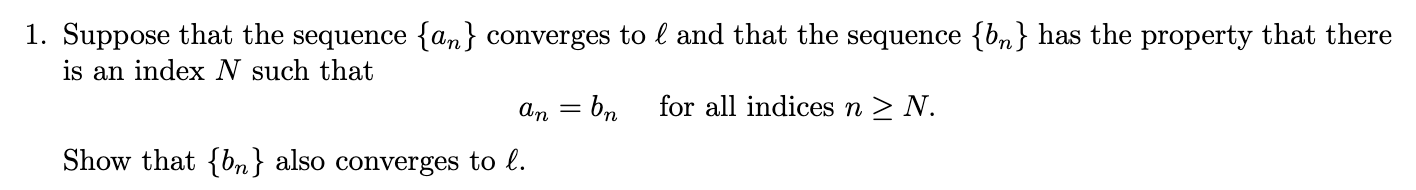
\includegraphics[width=15cm]{1.png}

\begin{proof}
  
\hfill

On the contrary, assume that a strictly increasing sequence $\{a_n\}$ has a peak index $a_m$, for some 
$m \in \NN$. By definition of strictly increasing, $a_{n+1} \geq a_n \ \forall \ n \in \NN$.
Since this works for all $n$, note that by definition of strictly increasing, $a_{m+1} \geq m$.
However, note that by definition of peak index
\[a_m > a_j \ \forall \ j \geq m \implies a_m > a_{m+1}\]
Thus, we've reached a contradiction since $a_{m+1} \geq m$ and $a_{m+1} < m$ obviously cannot
both be simulatenously true, and so a strictly increasing sequence has no peak indices.
\end{proof}

\newpage

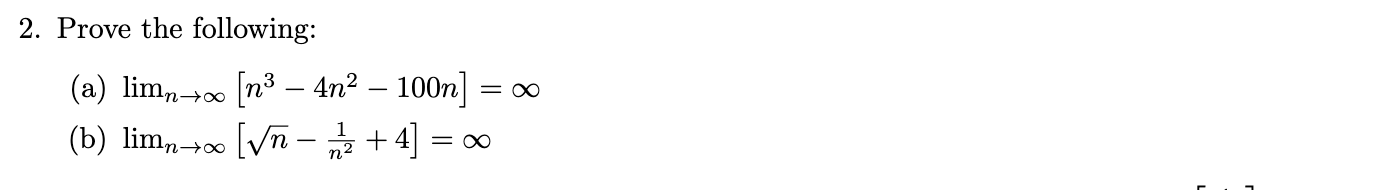
\includegraphics[width=15cm]{2.png}

\begin{proof}
  
\hfill

$\Longrightarrow$ Suppose we are given that the sequence $\{a_n\}$ does not converge to the 
number $a$. Therefore, by the definition of convergence, given some $\epsilon > 0$, 
we are not always guaranteed to be able to find $N \in \NN$ such that 
\[|a_n - a| < \epsilon \ \forall \ n \geq N\]
Choose one of these examples of $\epsilon$. Let us define the monotonically increasing sequence 
$\{n_k\} = \{i \ | \ |a_i - a| \geq \epsilon, i \geq N, i \in \NN\}$, or in plain English, all indices $i \geq N$
such that $|a_i - a| \geq \epsilon$.
Therefore, we have constructed a subsequence $\{a_{n_k}\}$ such that 
\[|a_{n_k} - a| \geq \epsilon \ \forall \ k\]
as desired.

\hfill

$\Longleftarrow$ The reverse direction is similar. Given $\epsilon > 0$ and some subsequence $\{a_{n_k}\}$, 
\[|a_{n_k} - a| \geq \epsilon \ \forall \ k\]
We WTS that $\{a_n\}$ does not converge to $a$. Suppose on the contrary, $\{a_n\}$ did converge to $a$. 
By definition of convergence, given any $\epsilon > 0$, we can find threshold $N \in \NN$ such that 
\[|a_n - a| < \epsilon \ \forall \ n \geq N\]
Note that this definition should work for all $\epsilon > 0$. Therefore,
let us choose the same $\epsilon$ as in the given statement. Note that $\{n_k\}$ is a monotonically increasing infinite sequence 
of natural numbers by definition of subsequence. Therefore, there exists some index in $\{n_k\}$ that is greater than or equal to
our threshold $N$. Let us denote this index $x$. Therefore, at index $x$, we have that $|a_x - a| \geq \epsilon$ by the given and $|a_x - a| < \epsilon$ by the definition of convergence. Clearly, this is a contradiction, 
and so $\{a_n\}$ cannot converge to $a$. 

\end{proof}

\newpage

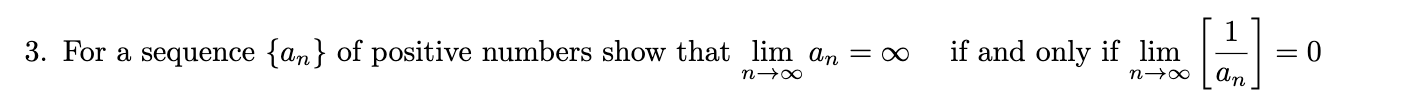
\includegraphics[width=15cm]{3.png}

\begin{proof}[Solution]

\hfill

\begin{enumerate}[a.]
  \item True. Assume on the contradiction that a bounded sequence $\{a_n\}$ had an unbounded subsequence $\{a_{n_k}\}$. 
  By definition of bounded, $\exists \ M \in \RR$ such that $|a_n| < M \ \forall \ n \implies -M < a_n < M \ \forall \ n$.
  If subsequence $\{a_{n_k}\}$ is unbounded then there some there exists some index $x \in \{n_k\}$ such that 
  $|a_x| \geq M$ because no scalar, not even $M$, is greater than the absolute value of all elements in the subsequence. 
  However $a_x$ is in the subsequence and also the sequence, so we have $|a_x| < M$ and $|a_x| \geq M$ simulatenously, which
  must be a contradiction, and so $\{a_{n_k}\}$ must also be bounded.
  \item True. On the contrary, suppose that the subsequence $\{x_{n_k}\}$ of a monotone sequence $\{x_n\}$ 
  was not monotone. WLOG assume the sequence is monotone increasing. By definition of monotone increasing, 
  $x_{n+1} \geq x_n \ \forall \ n$. Consider any sequence of indices $\{n_k\}$. Since the subsequence is not 
  monotone increasing, there must be some $x_{k'} < x_k, k', k \in \NN, k' > k$. However, note that 
  $x_{k'}$ and $x_k$ are also in the original sequence, which is monotone increasing and therefore 
  implies that $x_{k'} \geq x_k$. Thus, we have a contradiction, and so the subsequence of any monotone sequence 
  is also monotone.
  \item True. By a theorem presented in class, if a sequence $\{x_n\}$ converges to $a$, then 
  every subsequence $\{x_{n_k}\}$ also converges to $a$.
  \item False. Consider the sequence $\{a_n\} = \{\frac{1}{n}\}$ and the subsequent subsequence 
  $\{a_{n_k}\} = \{\frac{1}{n} \ | \ n \text{ is even}\}$. Note that $\{a_{n_k}\}$ converges to $1$, 
  but that the original subsequence we know does not converge. Therefore, we've found a counterexample.
\end{enumerate}
  
\end{proof}

\newpage

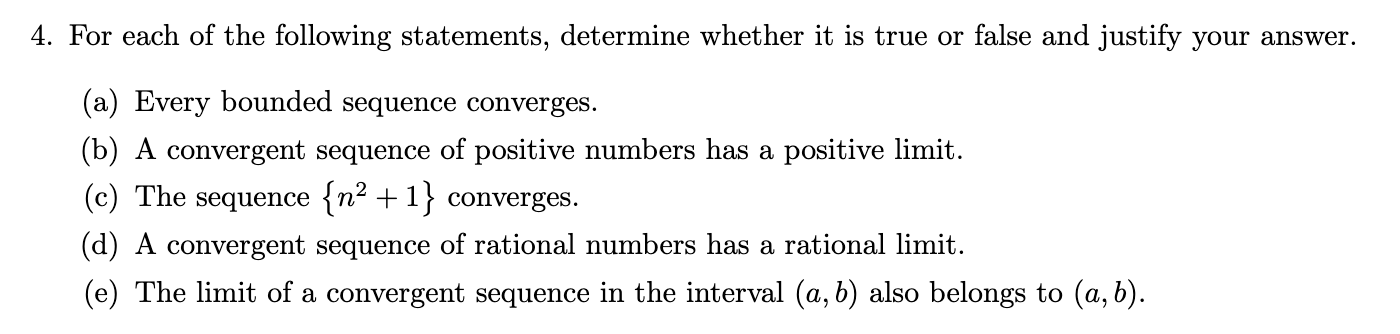
\includegraphics[width=15cm]{4.png}

\begin{proof}
  
\hfill

I claim the function is continuous at all points in the interval $[0, 1) \cup (1, 2]$. Essentially,
$f$ is continuous between $0$ and $2$ except for at $x = 1$, and we will show this over three parts.

\begin{enumerate}[a.]
  \item Select $x_0 \in [0, 1)$ and let the sequence $\{x_n\} \to x_0 \implies \underset{n\to\infty}{\lim}x_n = x_0$. We 
  WTS that $\underset{n\to\infty}{\lim}f(x_n) = f(x_0)$.
  Note that $\underset{n\to\infty}{\lim}x_n = \underset{n\to\infty}{\lim}11$ by definition of $f$. Further note that 
  $\underset{n\to\infty}{\lim}11 = 11 = f(x_0) \ \forall \ x \in [0, 1)$. Therefore, 
  $f$ is continuous on $[0, 1)$. 
  \item Now we will show that $f$ is discontinuous at $x_0 = 1$. Let $\{x_n\} \to x_0$ such that 
  the sequence approaches $x_0$ from the right, graphically. Note that 
  $\underset{n\to\infty}{\lim}f(x_n) = \underset{n\to\infty}{\lim}x_n = x_0 = 1 \neq 11 = f(x_0)$.
  Therefore, $\underset{n\to\infty}{\lim}f(x_n) \neq f(x_0)$ and so $f$ is discontinuous at $1$. 
  \item Finally, select $x_0 \in (1, 2]$ and let $\{x_n\} \to x_0$. Note that 
  $\underset{n\to\infty}{f(x_n)} = \underset{n\to\infty}{\lim}x_n = x_0 = f(x_0) \ \forall \ x_0 \in (1, 2]$. Therefore, 
  $f$ is continuous at all points in $(1, 2]$. 

\end{enumerate}

Putting everything together, $f$ is continuous on the interval $[0, 1) \cup (1, 2]$, as desired.
\end{proof}
\newpage

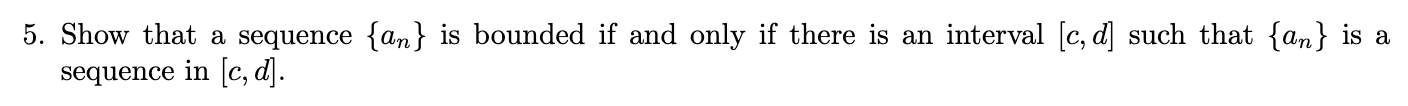
\includegraphics[width=15cm]{5.png}

\begin{proof}
  
\hfill

Assume on the contary that $f$ is continuous at $x_0 = 0$. Therefore, by definition of continuous at a point, 
\[\lim_{n\to\infty}f(x_n) = f(x_0) = f(0) = 0\]
Let the given sequence be $\{x_n\} = \{\frac{1}{n\pi}\} \to 0$ as $n\to\infty$ which we have discussed in class 
many times. Now consider 
\[\lim_{n\to\infty}f(x_n) = \lim_{n\to\infty}\sin(\frac{1}{\frac{1}{n\pi}}) = \lim_{n\to\infty}\sin(n\pi) \neq 0 \ \forall \ n\]
since $\sin(n\pi)$ oscillates. Since the function is never equal to $0$ and oscillates, it does not 
converge to 0, and therefore, we have reached a contradiction, and so $f$ must be discontinuous at $x_0=0$. 
\end{proof}
\newpage

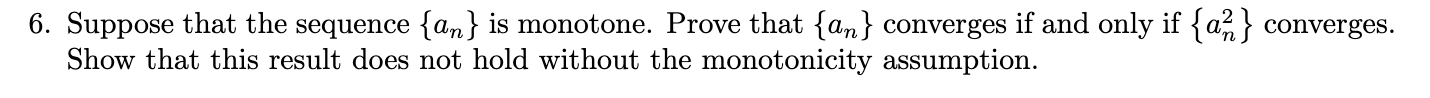
\includegraphics[width=15cm]{6.png}

\begin{proof}
  
\hfill

Note that $f$ is defined on $\RR$ and we WTS that it is continuous at $x = 0$. By 
Sequential Density of $\QQ$ and $\QQ^c$, we can find two sequences 
\[\{u_n\} \to 0, u_n \in \QQ \ \forall \ n\]
\[\{v_n\} \to 0, v_n \in \QQ^c \ \forall \ n\]
Trivially, since $f(v_n) = 0 \ \forall \ n \implies \underset{n\to\infty}{\lim}f(v_n) = f(x) = f(0) = 0$. 
Now, note that $\underset{n\to\infty}{\lim}f(u_n) = \underset{n\to\infty}{\lim}u_n = 0$
by construction. Even consider sequences that are mixed, in the sense that they contain elements that
are rational and elements that are irrational. All functional values of the irrational numbers are $0$, so it 
suffices to show that functional values of the rationals also converges to $0$ as the sequence of 
rationals converges to $0$. 
Therefore, since all index sequences that converge to $x=0$ implies that 
all image sequences converge to $f(x) = f(0) = 0$, then $f$ is continuous at $x=0$. 

\end{proof}
\newpage

\includegraphics[width=15cm]{7.png}

\begin{proof}
  
\hfill

We will show that this statement is false by counterexample. Let $a = -1$ and $b = 1$. 
Then the function 
\[f(x) = \begin{cases}
  1, 0 \leq x \leq 1\\
  -1, -1 \leq x < 0
\end{cases}\]
This function is plotted below. 

\includegraphics[width=15cm]{step.png}

Clearly, the domain of $f$ is $[-1, 1]$, the max of $f$ is 1 and the min of $f$ is $-1$, and $f$
is not continuous at. We will prove this rigorously. Let $x_0 = 0$ and let there be 
a sequence $\{x_n\} \to 0$, specifically approaching $0$ from the left side graphically. 
Note that $\underset{n\to\infty}{\lim}f(x_n) = -1 \neq f(x_0) = f(0) = 1$. Therefore, 
$f$ is not continuous at $x_0 = 0$, and we proved the given statemtent false.   

\end{proof}
\newpage

\includegraphics[width=15cm]{8.png}

\begin{proof}
  
\hfill

\begin{enumerate}[a.]
  \item Consider $f: (a, b) \to \RR$ such that $f(x) = \frac{1}{x-a}$. $f$ is continuous because $x \neq a \implies$ the 
  denominator is never $0$ and so this function is defined everywhere. Consider the sequence 
  $\{x_n\} \to a$, which exists by density of $\RR$. Now consider 
  \[\lim_{n\to\infty}f(x_n) = \lim_{n\to\infty} \frac{1}{x_n - a} = \infty\]
  Theerefore, $f$ diverges on this interval and is therefore unbounded above. 

  \item Now consider $f: (a, b) \to \RR$ such that $f(x) = x$. Note that $f$ is bounded above by $b$ on the
  interval $(a, b)$. Suppose on the contrary that $f$ attains a maximum value. By definition of 
  maximum, there is $x_0 \in (a, b)$ such that $f(x_0) \geq f(x) \ \forall \ x \in (a, b)$. 
  Note that $f(x_0) = x_0$. Take the midpoint between $x_0$ and $b$, given by $\frac{x_0 + b}{2}$. 
  Note that $f(\frac{x_0 + b}{2}) = \frac{x_0 + b}{2}$. Since $b$ is guaranteed to be 
  larger than $x_0$, since $x_0 \in (a,b)$, then we know that 
  \[\frac{x_0 + b}{2} > x_0\]
  and thus, $x_0$ cannot be a maximum for $f$, and so we have our contradiction. Therefore, while 
  $f$ is bounded above, it does not attain a maximum value.
\end{enumerate}


\end{proof}
\end{document}

